\documentclass{beamer}
\usepackage[utf8]{inputenc}   
\usepackage[T1]{fontenc}       
\usepackage[polish]{babel}     
\setbeamertemplate{caption}{\insertcaption}

\usetheme{CambridgeUS}

\title{Wpływ gier Dark Souls na człowieka}  %1slajd
\author{Dawid Szokało}
\date{18 Stycznia 2025}

\begin{document}

\begin{frame}
    \titlepage
\end{frame}

\begin{frame}{Spis treści:}  %2slajd

\begin{enumerate}
 \item Wstęp
    \item Charakterystyka gier \glqq Dark Souls\grqq
        \begin{itemize}
      \item Mechanika gier Dark Souls
      \item Butelka Estusa
       \item Narracja i świat przedstawiony
        \end{itemize}

    \item Wpływ gier \glqq Dark Souls\grqq na psychikę i emocje graczy
      \begin{itemize}
      \item Frustracja i satysfakcja z pokonywania trudności
      \item Stres
       \item Rozwijanie wytrwałości i cierpliwości
        \end{itemize}

    \item Wpływ gier \glqq Dark Souls\grqq na interakcje społeczne
     \begin{itemize}
      \item Wiadomości pozostawione przez graczy
      \item Przyzywanie innych graczy
       \item Inwazja
       \item Współpraca w trybie online
       \item Rywalizacja w trybie online
       \item Kultura współpracy
        \end{itemize}

    \item Podsumowanie
\end{enumerate}
\end{frame}

\begin{frame}{1.Wstęp}  %3slajd
\small Seria gier Dark Souls, stworzona przez japońskie studio FromSoftware pod nadzorem Hidetaki Miyazakiego, zdobyła międzynarodową sławę, stając się jednym z najbardziej wpływowych i wymagających tytułów w historii gier komputerowych. Od momentu debiutu w 2011 roku, seria  zdobyła serca wielu graczy,  wpływając na nich, jak i na  kulturę gier. Co czyni tę grę  tak wyjątkową? Posiada nieliniową fabułę, jest trudna, a jej wyjątkowa mechanika uzależnia.
 \begin{figure}
    \centering
        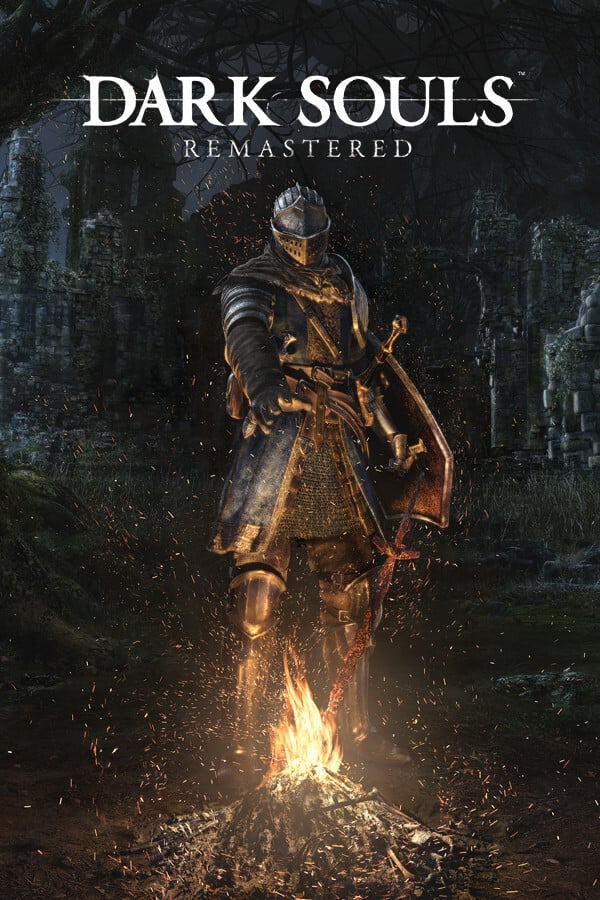
\includegraphics[width=6cm,height=5.5cm]{ds1.jpg}
 
    \end{figure}

\end{frame}


\begin{frame}{2.Charakterystyka gier \glqq Dark Souls\grqq} %4slajd
\begin{columns}
% Column 1
\begin{column}{0.5\textwidth}
\small     Seria  Dark Souls  to fabularne gry akcji, których akcja rozgrywa się w otwartym świecie. Gry te wyróżniają się ogromnym poziomem trudności oraz brakiem normalnego systemu wskazówek. Oprócz standardowych porad takich jak walka, czy blok ciosu tarczą,  gracze muszą odkrywać świat na własną rękę, co dla niektórych graczy może być frustrujące a dla innych satysfakcjonujące. Jednym z kluczowych elementów w owych grach jest ich trudność, którą gracze pokochali. Gra nie daje graczom łatwych ścieżek, czy wskazówek. Każda decyzja może prowadzić do śmierci, a ona nie jest tylko karą, ale także ważnym elementem samej gry.

\end{column}
% Column 2    
\begin{column}{0.5\textwidth}
    \begin{figure}
    \centering
        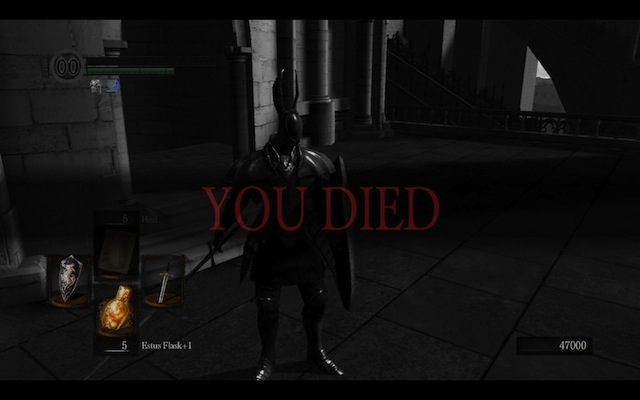
\includegraphics[width=5.5cm,height=5cm]{You died ds.jpg}
 
    \end{figure}
\end{column}
\end{columns}

\end{frame}

\begin{frame}{Mechanika gier \glqq Dark Souls\grqq} %5slajd
\begin{columns}
% Column 1
\begin{column}{0.5\textwidth}
\small      Bardzo kluczową częścią mechaniki w tej serii jest wytrzymałość. Jej zarządzanie wpływa na całą naszą rozgrywkę. Każda akcja, ruch, czy uderzenie zabiera nam kawałek wytrzymałości. Po zużyciu całej wytrzymałości gracz staje się zupełnie bezbronny. Nie może wykonać uniku, ataku i innych rzeczy związanych z wytrzymałością oprócz czekania, aż ta się zregeneruje. Złe nadzorowanie tego elementu może skończyć się utratą kawałka paska życia lub nawet śmiercią.

\end{column}
% Column 2    
\begin{column}{0.5\textwidth}
    \begin{figure}
    \centering
        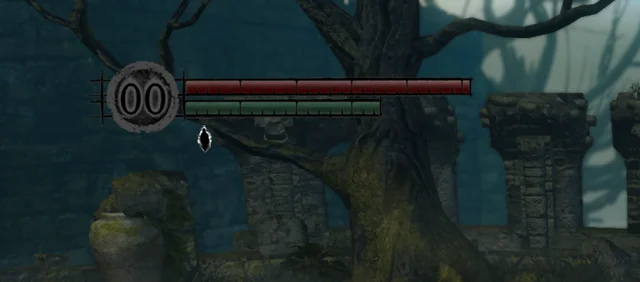
\includegraphics[width=5.5cm,height=5cm]{stamina.jpg}
 
    \end{figure}
\end{column}
\end{columns}

\end{frame}

\begin{frame}{Butelka Estusa} %6slajd

 \begin{figure}
    \centering
        
\includegraphics[width=6cm,height=5cm]{Estus.jpg}
 
    \end{figure}
\small Gracz na początku każdej gry z serii dostaje wybitnie ważny przedmiot, który będzie przydatny podczas całej naszej podróży. Butelka Estusa, bo o tym przedmiocie mowa, ma ograniczoną ilość użyć oraz za każdym użyciem przywraca kawałek paska życia postaci. Ilość użyć tego przedmiotu resetuje się za każdym razem, gdy gracz będzie odpoczywał przy ognisku.

\end{frame}

\begin{frame}{Narracja i świat przedstawiony} %7slajd
\begin{columns}

\begin{column}{0.5\textwidth}
    \begin{figure}
    \centering
        \includegraphics[width=5.5cm,height=5cm]{Ds3 świat.jpg}
 
    \end{figure}
\end{column}

\begin{column}{0.5\textwidth}
\small     Fabuła w serii Dark Souls nie jest bezpośrednio opowiedziana graczowi, a świat jest mroczny i pełen tajemnic. Historię gry można odkryć za pomocą eksploracji świata, rozmawiając z NPC-ami lub czytając opisy przedmiotów. Jak powiedział sam Miyazaki, celem było stworzenie gry nieliniowej, w której gracze byliby skupieni na rozgrywce zamiast na samej fabule.  Taka forma narracji zmusza graczy chcących lepiej poznać świat i jego historię do odkrywania kolejnych to sekretów ukrytych po całym świecie gier i interakcji z postaciami.

\end{column}
\end{columns}

\end{frame}

\begin{frame}{3.Wpływ gier  \glqq Dark Souls\grqq na psychikę i emocje graczy} %8slajd
\begin{columns}
% Column 1
\begin{column}{0.5\textwidth}
\normalsize \textbf{ Frustracja i satysfakcja z pokonywania trudności.}

\small    Wysoka trudność potrafi wywołać frustrację. Zwłaszcza, gdy gracze umierają z powodu ich błędów czy też trudnych przeciwników. Jednak pokonywanie trudności jakie napotykamy w serii Dark Souls jest źródłem satysfakcji. Po każdym nieudanym ataku, uniku czy nieudanej walce uczymy się coraz więcej o przeciwnikach co pozwala nam zbliżyć się do upragnionego  zwycięstwa. Te uczucie sukcesu, które uzyskujemy po wielu błędach i porażkach sprawia, że te gry są tak uzależniające.
\end{column}

% Column 2    
\begin{column}{0.5\textwidth}
    \begin{figure}
    \centering
        \includegraphics[width=5.5cm,height=5cm]{Satysfakcja.jpg}
 
    \end{figure}
\end{column}
\end{columns}

\end{frame}

\begin{frame}{Stres} %9slajd
\begin{columns}
% Column 1
\begin{column}{0.5\textwidth}
\small      Każdy ruch w grze może skutkować śmiercią postaci, a w grze brakuje prostych wskazówek. Zmusza to graczy do ciągłej analizy otoczenia, przewidywania niebezpieczeństw i dostosowywania się do dynamiki gry.  Takie rozwiązanie powoduje wzrost poziomu stresu u graczy. W Dark Souls jest on zbalansowany przez uczucie satysfakcji za każdym razem, gdy pokona się trudnego przeciwnika.
\end{column}

% Column 2    
\begin{column}{0.5\textwidth}
    \begin{figure}
    \centering
        
\includegraphics[width=5.5cm,height=5cm]{stres.jpg}
 
    \end{figure}
\end{column}
\end{columns}

\end{frame}

\begin{frame}{Rozwijanie wytrwałości i cierpliwości}  %10slajd
\small Gry z omawianej serii są głównie przeznaczone dla wytrwałych graczy, ponieważ wymagają od graczy uczenia się na błędach, powtarzania wielokrotnie pewnych sekwencji i bycia cierpliwym. Hidetaka Miyazaki w jednym z wywiadów podczas premiery pierwszej odsłony trylogii Dark Souls przyznał, że od poprzedniej jego gry pod tytułem Demon Souls format uczenia się na błędach dalej pozostanie.
\centering
    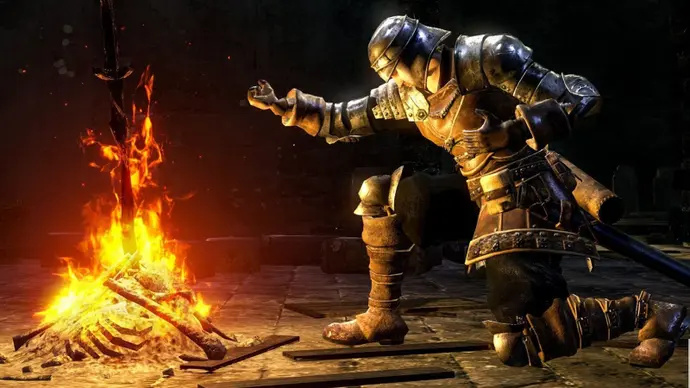
\includegraphics[width=8cm,height=5cm]{ognisko.jpg}

\end{frame}

\begin{frame}{4.Wpływ gier \glqq Dark Souls\grqq na interakcje społeczne}  %11slajd
\small Choć Dark Souls  to gry głównie single-player, to zawierają jednak elementy pozwalające graczom wchodzić ze sobą w interakcje. Systemy te wpływają na sposób, w jaki gracze łączą się i wymieniają doświadczeniami.

\begin{figure}
\centering
    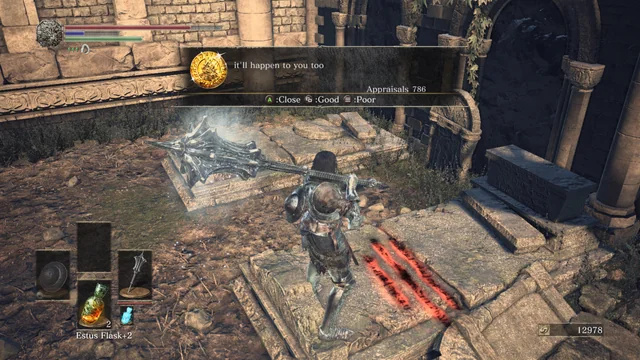
\includegraphics[width=7cm,height=5cm]{wiadomość.jpg}
    \caption{Wiadomości pozostawione przez graczy}

\end{figure}
\end{frame}

\begin{frame} %12slajd
\begin{columns}
% Column 1
\begin{column}{0.5\textwidth}
\begin{figure}
\centering
    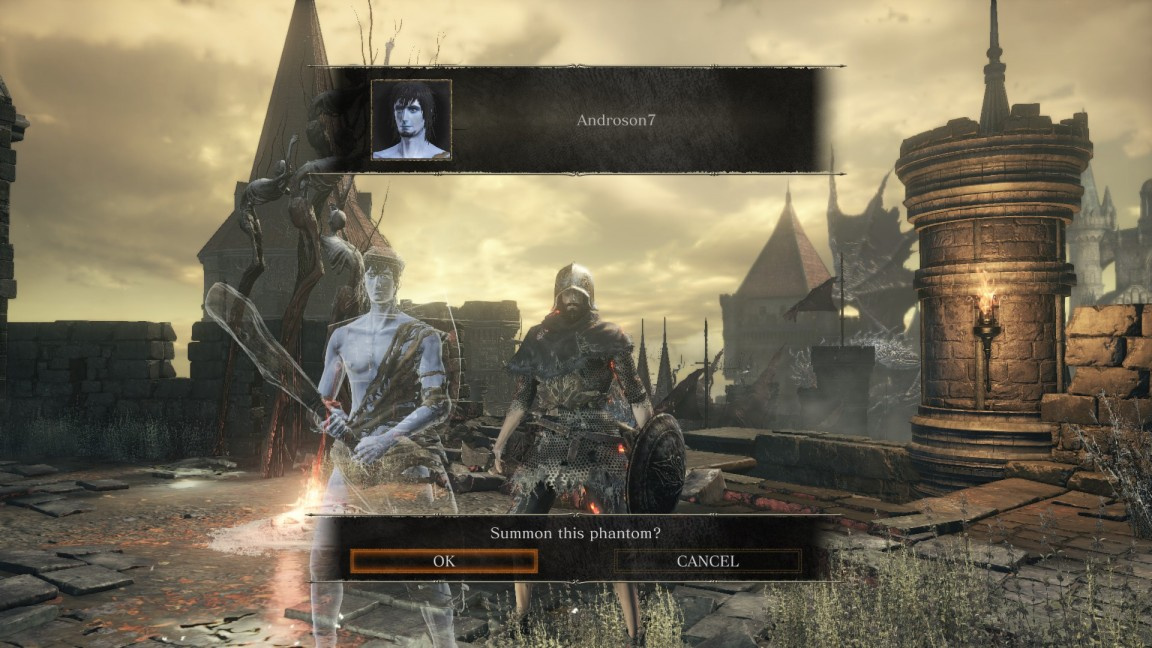
\includegraphics[width=6cm,height=5cm]{przyzywanie.jpg}
    \caption{Przyzywanie innych graczy}
\end{figure}
\end{column}

% Column 2    
\begin{column}{0.5\textwidth}
\begin{figure}
\centering
    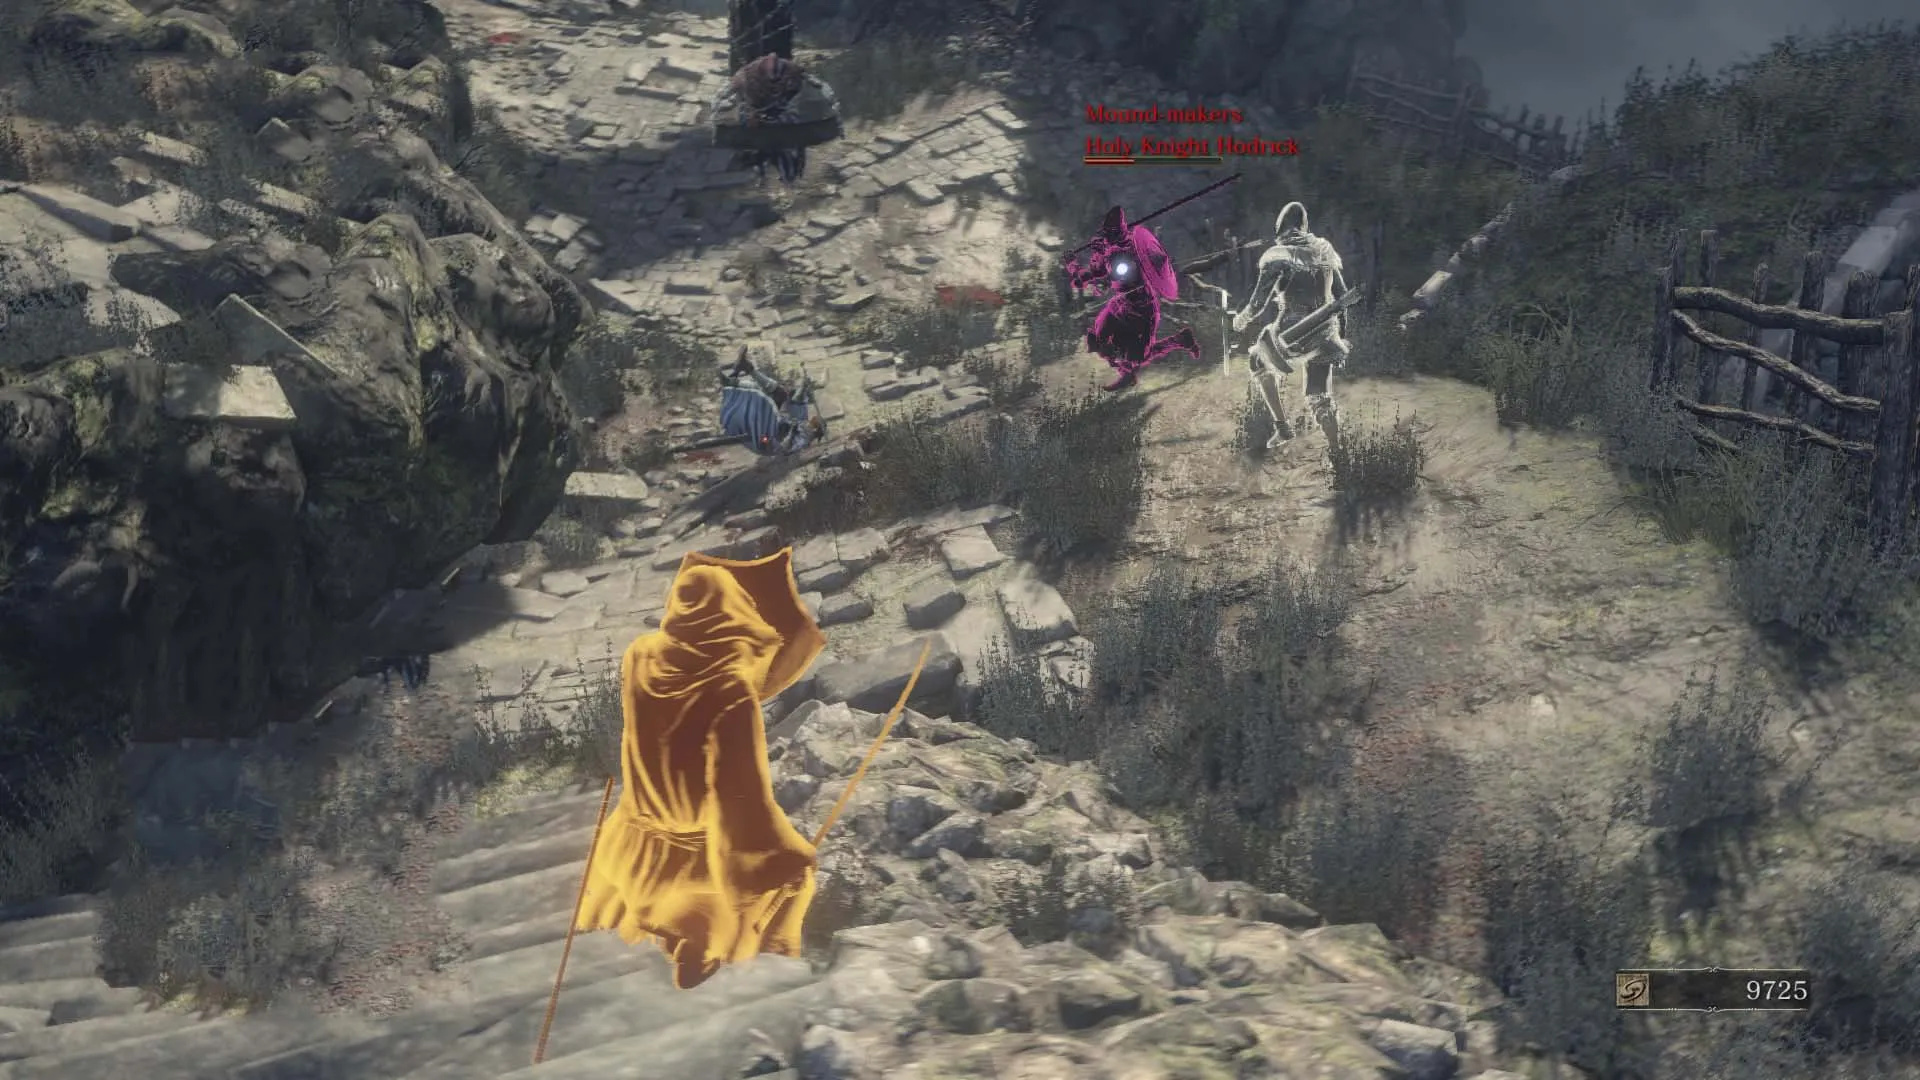
\includegraphics[width=6cm,height=5cm]{inwazja.jpg}
    \caption{Inwazja}
    
\end{figure}
\end{column}
\end{columns}
\end{frame}

\begin{frame}{Współpraca w trybie online} %13slajd
\begin{columns}

\begin{column}{0.5\textwidth}
    \begin{figure}
    \centering
        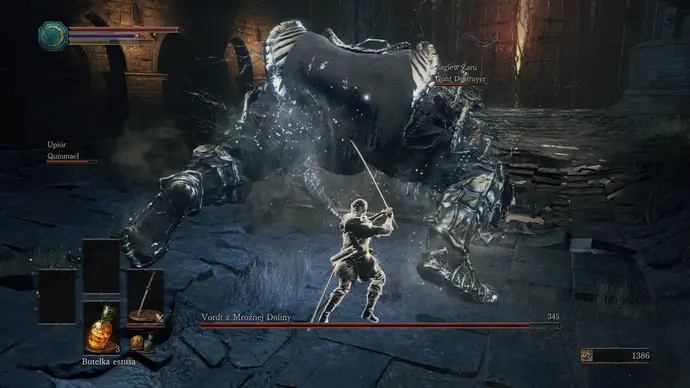
\includegraphics[width=5.5cm,height=5cm]{pomoc.jpg}
 
    \end{figure}
\end{column}

\begin{column}{0.5\textwidth}
\small     W grach tej serii istnieją aspekty zachęcające graczy do współpracy. Jednym z nich jest zostawianie wiadomości. Gracze mogą używać wybranych przez grę słów aby tworzyć na ziemi wiadomości, które mogą na przykład pomóc innym znaleźć ukryte przejście w ścianie czy mogą ostrzegać przed niespodziewanym przeciwnikiem czekającym tuż za rogiem. Innym elementem jest pomaganie innym w walce z trudnymi bossami. Seria Dark Souls pozwala graczom przyzywać innych graczy z tej samej frakcji by ci pomogli im w walce z bossem. Zazwyczaj znaki do przywołania innych ludzi są umiejscowione blisko wejścia na arenę z danym bossem. 

\end{column}
\end{columns}
\end{frame}

\begin{frame}{Rywalizacja w trybie online} %14slajd
\begin{columns}
% Column 1
\begin{column}{0.5\textwidth}
\small      Kolejnym kluczowym aspektem w tej serii  jest rywalizacja. W trybie PvP jeden z graczy może „najechać” świat innego gracza w dowolnym momencie. W tym momencie oboje próbują pokonać się nawzajem i wygrany otrzymuje przedmiot potrzebny do ulepszenia poziomu frakcji, w której się znajduje. Forma PvP to nie jedyny sposób na rywalizację w serii Dark Souls. Rywalizacja może też polegać na robieniu przeróżnych wyzwań, które mogą być wymagające. Najpopularniejszym z nich jest przejście gry bez żadnej śmierci, a to może być momentami trudne ze względu na swoje błędy podczas walki lub przypadkowy upadek z wysokości. 
\end{column}

% Column 2    
\begin{column}{0.5\textwidth}
    \begin{figure}
    \centering
        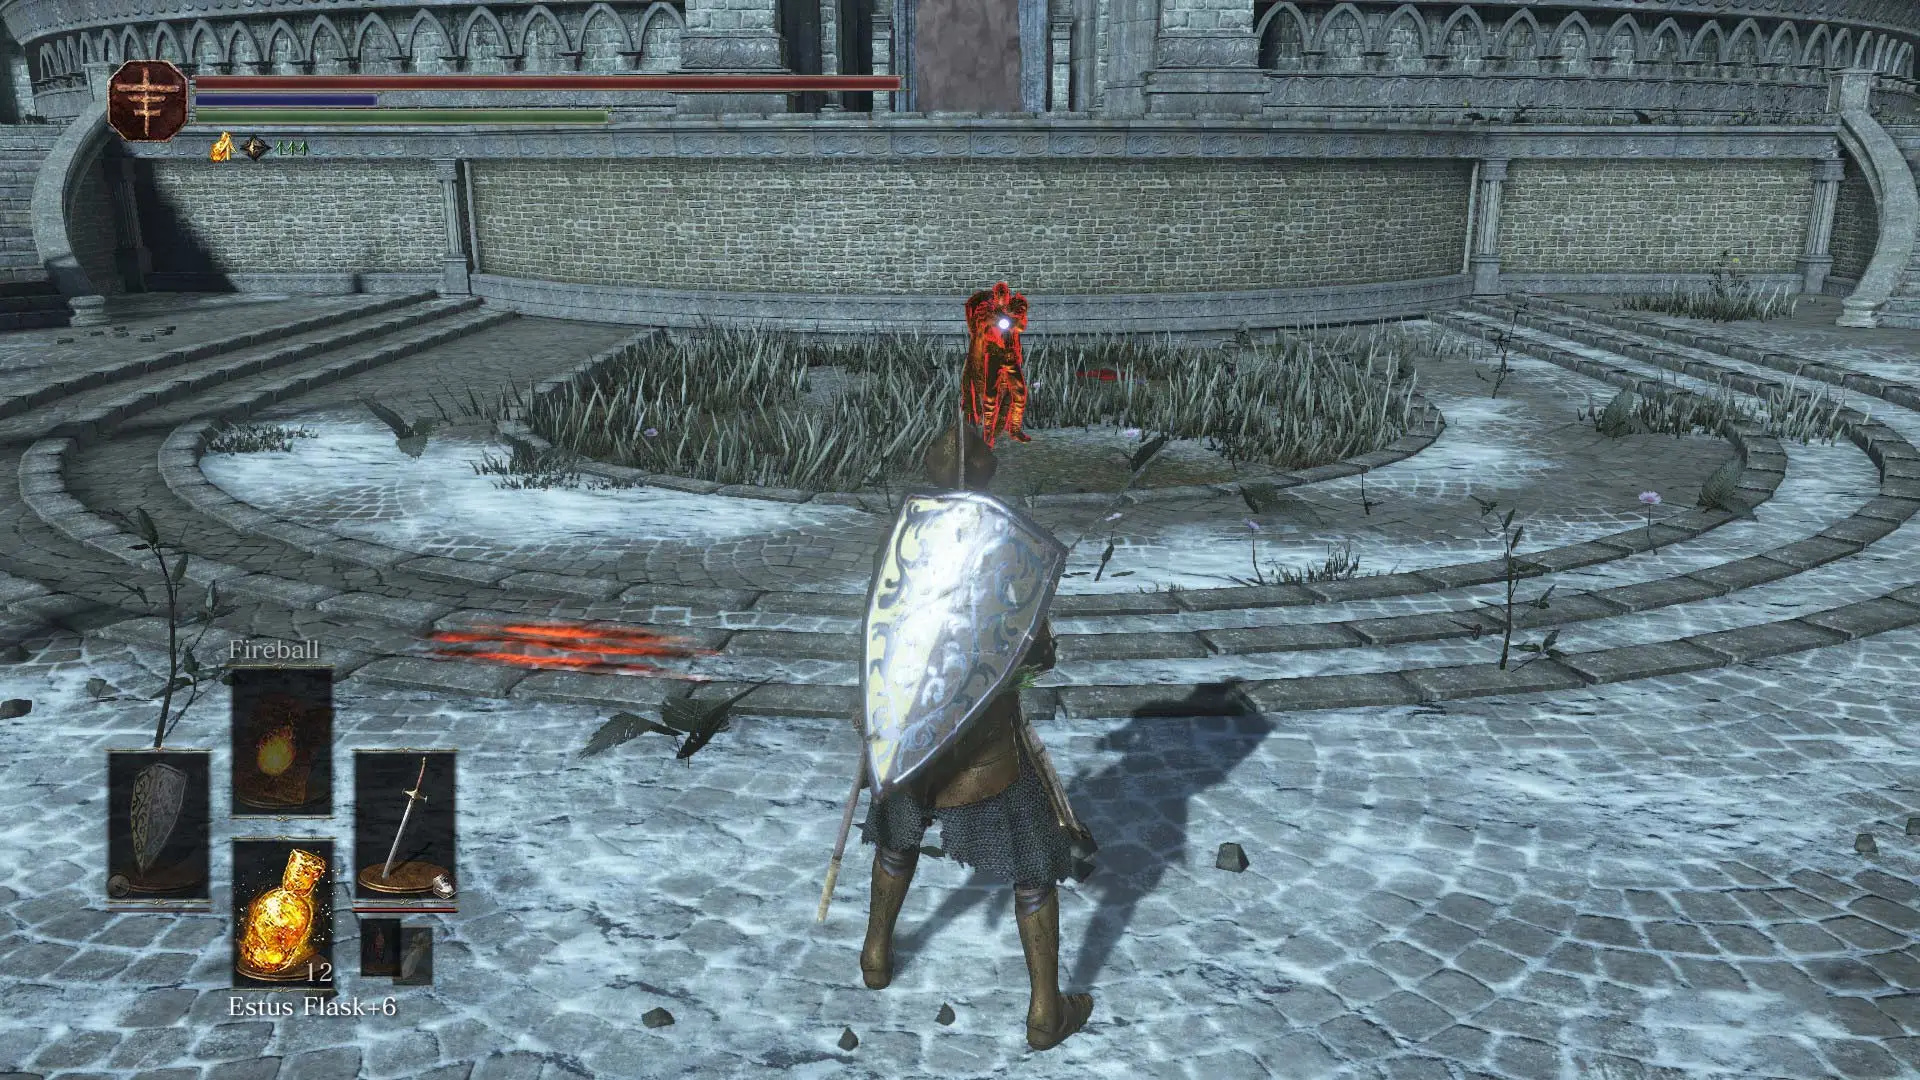
\includegraphics[width=6cm,height=5.5cm]{pvp.jpg}
 
    \end{figure}
\end{column}
\end{columns}
\end{frame}


\begin{frame}{Kultura współpracy}  %15slajd
\small Istnieje silna kultura wzajemnej pomocy wśród graczy Dark Souls, polegająca na dzieleniu się swoimi poradami, strategiami i doświadczeniami. Pomoc innym graczom staje się nieodłączną częścią gier, która tworzy przestrzeń przyjaznej społeczności. Mimo rywalizacji i  indywidualnych osiągnięć, gracze pokazują, że nadal można wspierać innych.

 \begin{figure}
    \centering
        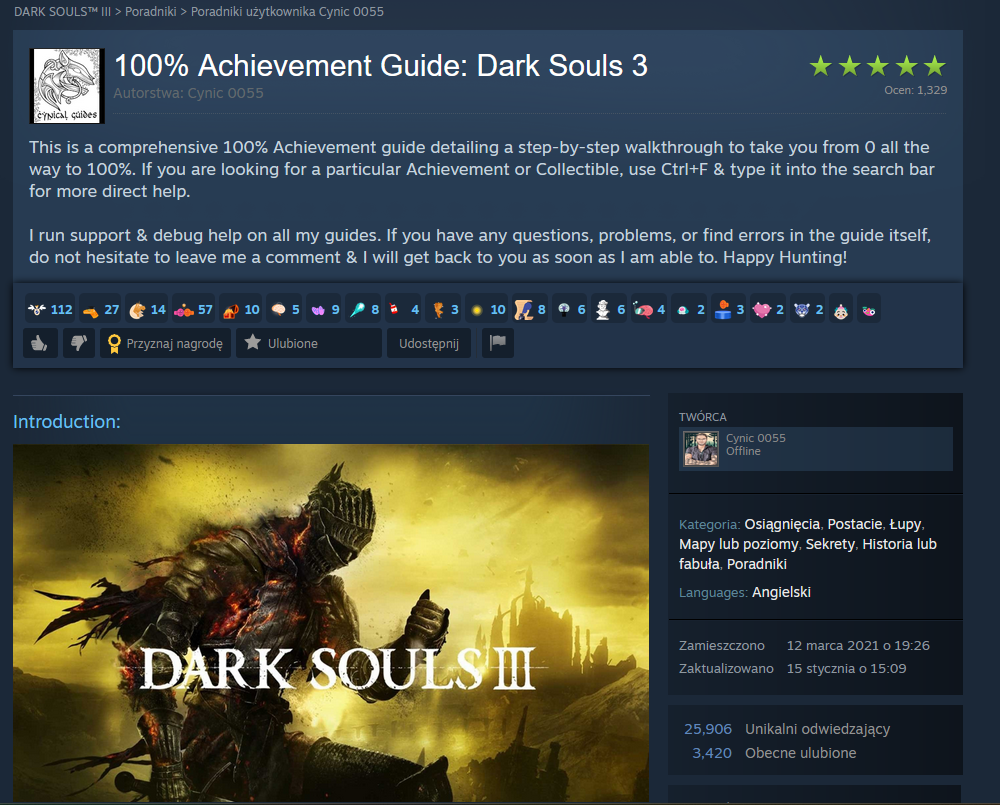
\includegraphics[width=6cm,height=5.5cm]{poradnik.png}
 
    \end{figure}
\end{frame}

\begin{frame}{5.Podsumowanie}  %16slajd
\small Seria Dark Souls ogromnie wpływa na psychikę, emocje i interakcje społeczne graczy. Wprawdzie poziom trudności może prowadzić do frustracji, ale jednocześnie seria daje graczom poczucie satysfakcji i pomaga im wzmocnić zdolność radzenia sobie z wyzwaniami. Interakcje społeczne pomagają graczom budować wspólną więź i zachęcają do współpracy.  Gry z serii Dark Souls są przykładem jak gry komputerowe mogą wpływać na graczy pozytywnie, jak i negatywnie.
\end{frame}

\begin{frame}
		\frametitle{Bibliografia}
			\begin{thebibliography}{99}
			\bibitem{1}
			https://www.xxlgamer.pl 
			\bibitem{2}
			https://zonaduscae.wordpress.com/2017/06/24/dark-souls-facilis-descensus-averno/
                               \bibitem{3}
			https://www.reddit.com/r/darksouls/comments/1arhbnc/
			\bibitem{4}
			https://darksoulspl.wiki.fextralife.com 
                                \bibitem{5}
			https://medium.com/@couriereight/games-at-the-end-of-the-world-edbcd015e3f8 
			\bibitem{6}
			https://plusydlabiznesu.pl/aktualnosci/2672/co-piaty-polak-codziennie-stresuje-sie-w-pracy 
                                \bibitem{7}
			https://www.controlling-24.pl/artykul/zarzadzanie-satysfakcja-klienta
		\end{thebibliography}
	\end{frame}

\begin{frame}
		\frametitle{Bibliografia}
			\begin{thebibliography}{99}
			\bibitem{1}
			https://www.eurogamer.net/bonfires-are-still-my-favourite-fromsoftware-idea
			\bibitem{2}
			https://www.reddit.com/r/fromsoftware/comments/
                               \bibitem{3}
			https://www.vg247.com/dark-souls-3-the-complete-guide-to-summoning-and-playing-co-op
			\bibitem{4}
			 https://www.polygon.com/2016/4/20/11466700/
                                \bibitem{5}
			https://www.eurogamer.pl/dark-souls-3-multiplayer-atakowanie-graczy-wzywanie-pomocy 
			\bibitem{6}
			https://www.polygon.com/2016/5/3/11566388/dark-souls-3-invasions-explained-cracked-red-eye-orb-summon-sign-colors-covenants 
                                \bibitem{7}
			https://steamcommunity.com/sharedfiles/filedetails/?id=2422780990 
		\end{thebibliography}
	\end{frame}
\end{document}